\begin{center}
Общее представление о системе
\end{center}

\vspace{\baselineskip}

FreeHackQuest (FHQ) -- это платформа для обучения, проведения практических занятий и соревнований по компьютерной безопасности в формате тестирования на проникновение внутри среды, моделирующей работу информационной инфраструктуры организации. FHQ включает в себя учебник, различные задачи для решения, связанные с администрированием, криптографией, компьютерно-криминалистической экспертизой, стеганографией и многими дргуими направлениями информационной безопасности.\par

\begin{center}
Основные компоненты системы
\end{center}

\vspace{\baselineskip}

FreeHackQuest представляет собой клиент–серверную многофункциональную систему с подсистемами и состоит из следующих основных компонентов:
\begin{enumerate}
\item Уровень 1: Сервер -- отвечает за обработку запросов со стороны клиента.
\item Уровень 1: LXD (сервер виртуальных машин) -- предназначен для размещения контейнеров, необходимых, для изолированного выполнения сервисов с уязвимостями.
\item Уровень 1: MySQL (сервер баз данных) -- отвечает за хранение и предоставление информации.
\item Уровень 1: Клиент -- отвечает за формирование запросов подсистеме сервера и представление ответов со стороны сервера.
\item Уровень 1: Административный клиент -- отвечает за управление системой.
\end{enumerate}

\vspace{\baselineskip}

Структура системы представлена на рисунке \ref{img:1}.

\begin{figure}[h!]
        \centering
        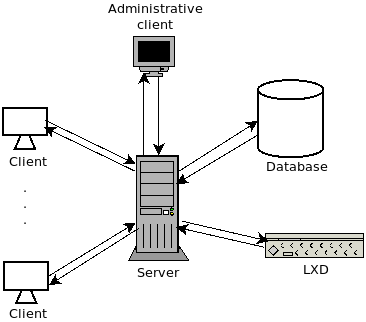
\includegraphics[width=0.65\textwidth]{1}
        \caption{Структура системы}
        \label{img:1}
\end{figure}

\begin{center}
Описание стека технологий системы
\end{center}

Архитектура клиент-сервер определяет лишь общие принципы взаимодействия между компьютерами, детали взаимодействия определяют различные протоколы. Данная концепция нам говорит, что нужно разделять машины в сети на клиентские, которые делают запрос, и на серверные, которые отвечают на него. При этом взаимодействие всегда начинает клиент, а правила, по которым происходит взаимодействие описывает протокол.\par
За взаимодействие между сервером и клиентами, в том числе с административным клиентом, отвечает протокол WebSocket (WS/WSS). Данный протокол связи поверх TCP-соединения предназначен для обмена сообщениями между браузером и веб-сервером в режиме реального времени.\par
MySQL как СУБД, если рассматривать её в рамках клиент-серверной архитектуры, является прежде всего программой-сервером, который может получать от различных клиентов, задачи по работе с данными (посредством SQL-запросов).\par 
Этими клиентами могут быть:
\begin{itemize}
\item собственная-программа клиент работающая в командной строке;
\item скрипт, написанный на каком-нибудь языке программирования, например, на PHP (так называемый <<запрос из приложения>>);
\item программа для работы с данными в графическом интерфейсе.\par
\end{itemize}
\vspace{\baselineskip}

Взаимодействие c e-mail осуществляется посредством SMTP-протокола -- протокола для исходящей связи по электронной почте. Простой протокол передачи почты (SMTP), используется для связи с удаленным сервером и последующей отправки сообщений с локального клиента на удаленный сервер, и в конечном итоге на сервер получателя сообщений. SMTP используется исключительно для отправки сообщений.\par
Если выполняется условие if enabled lxd, то сервер обращается к серверу виртуальных машин (LXD).\par
\vspace{\baselineskip}

\begin{center}
LXD
\end{center}

Система виртуализации необходима для изолированного выполнения сервисов с уязвимостями, так как участники могут скомпрометировать машину, на которой развернута моделируемая инфраструктура организации. Система виртуализации должна обладать сетевым управлением, такое требование позволяет размещать контейнеры на отдельной от backend сервера машине. Например, у хостинг-провайдеров можно арендовать необходимые вычислительные мощности на время проведения практики и обучения.\par
В качестве системы виртуализации выбран LXD (LXC). LXD это то, что называется легковизор. Ядром LXD является демон, который предлагает API REST для управления контейнерами подобно виртуальным машинам. Чтобы создавать, управлять и мониторить множество уязвимых сервисов с определенными настройками сети прямо в административной странице FreeHackQuest, появилась необходимость интеграции FreeHackQuest с LXD.\par

\begin{center}
Continuous Integration
\end{center}

Continuous Integration — это практика разработки программного обеспечения, которая заключается в слиянии рабочих копий в общую основную ветвь разработки несколько раз в день и выполнении частых автоматизированных сборок проекта для скорейшего выявления потенциальных дефектов и решения интеграционных проблем. В обычном проекте, где над разными частями системы разработчики трудятся независимо, стадия интеграции является заключительной. Она может непредсказуемо задержать окончание работ. Переход к непрерывной интеграции позволяет снизить трудоёмкость интеграции и сделать её более предсказуемой за счет раннего обнаружения и устранения ошибок и противоречий. Основным преимуществом является сокращение стоимости исправления дефекта, за счёт раннего его выявления. \par
Зачем нужна непрерывная интеграция? Раньше разработчики одной команды могли в течение долгого времени работать изолированно и объединяли свои изменения с основной частью проекта только по завершении собственной работы. Это делало слияние кода сложной и трудоемкой задачей, к тому же ошибки накапливались и не исправлялись в течение долгого времени. Такие факторы затрудняли быструю доставку обновлений пользователям. CI упростила эту задачу. \par
Как работает непрерывная интеграция? При непрерывной интеграции разработчики часто подтверждают записи в совместно используемый репозиторий, используя систему контроля версий, например, Git. Перед каждым подтверждением записи разработчики могут запускать локальные модульные тесты программного кода в качестве дополнительного уровня проверки перед интеграцией. Сервис непрерывной интеграции автоматически выполняет сборку и запуск модульных тестов для изменений кода, что позволяет моментально выявлять ошибки. \par

Преимущества:
\begin{itemize}
\item более продуктивная разработка - непрерывная интеграция повышает производительность вашей команды за счет освобождения разработчиков от ручной работы и стимуляции подходов, которые помогают уменьшить количество ошибок и дефектов в версиях ПО для конечных пользователей;
\item быстрое обнаружение и устранение ошибок - за счет более частого и всестороннего тестирования ваша команда сможет выявлять и устранять ошибки заблаговременно, до того, как они перерастут в серьезные проблемы;
\item быстрая доставка обновлений - непрерывная интеграция дает возможность вашей команде быстрее и чаще доставлять обновления конечным пользователям.
\end{itemize}
\vspace{\baselineskip}

Идеальный процесс выглядит примерно так:
\begin{itemize}
\item разработчик отправляет код в центральный репозиторий;
\item на сервере непрерывной интеграции изменения объединяются с основным кодом, выполняются юнит – тесты и всё заливается на стэйжинг среду;
\item в стэйжинг среде приложение тестируется;
\item дальше всё проверяется для попадания на продакшен;
\item развёртывание на продакшене.
\end{itemize}
\vspace{\baselineskip}

\begin{center}
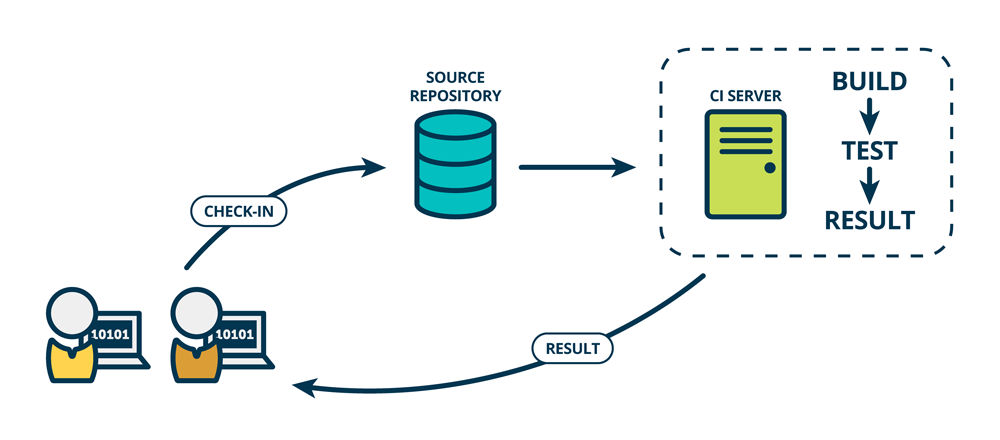
\includegraphics[width=0.65\textwidth]{ci}\\
Рисунок -- Continous Integration\\
\end{center}

